\documentclass[hperref={pdfpagelabels=false}]{beamer}

\usefonttheme[onlymath]{serif}
\usepackage{lmodern}
\usepackage[T1]{fontenc}
\usepackage[utf8]{inputenc}
\usepackage{hyperref}
\usetheme{default}
\usepackage{physics}
\usepackage{caption}
% \captionsetup{font=scriptsize,labelfont=scriptsize}

\begin{document}

\title
{Computing project: Neutron star}

\subtitle{Neutron star modelled as pure Fermi gas with nucleon interaction}

\author
{Luis Caceres Cueva \and Tomoi Goto}

\institute
{
    School of Phsyics and Astronomy\\
    The University of Manchester
}
\date
{May 8, 2019}

\begin{frame}
 \titlepage
\end{frame}

\begin{frame}
 \frametitle{Structure equations}
 Newtonian structure equation is
 \begin{align*}
  \dv{p}{r}&=-\frac{G\rho M}{r^{2}}\\
  \dv{M}{r}&=4\pi r^{2}\rho.
 \end{align*}
 
General Relativistic structure equation (TOV equation) is
 \begin{align*}
  \dv{p}{r}&=-\frac{G\rho M}{r^{2}}\qty[1+\frac{p}{\epsilon}]\qty[1+\frac{4\pi r^{3}p}{Mc^{2}}]\qty[1-\frac{2GM}{c^{2}r}]^{-1}\\
  \dv{M}{r}&=4\pi r^{2}\rho.
 \end{align*}
\end{frame}

\begin{frame}
 \frametitle{Fermi gas model}
 We define the dimensionless quantity \[x\equiv\frac{\hbar k_{F}}{mc}.\]
 
 Hence, we can write the relevant quantities
 \begin{align*}
  n&=n_{0}x^{3},&n_{0}&=\frac{m^{3}c^{3}}{3\pi^{2}\hbar^{3}},\\
  \rho&=\rho_{0}x^{3},&\rho_{0}&=\frac{m^{4}c^{3}}{3\pi^{2}\hbar^{3}},\\
  \epsilon&=\epsilon_{0}x^{3}I(x),&\epsilon_{0}&=\frac{m^{4}c^{5}}{3\pi^{2}\hbar^{3}},\\
  p&=\frac{1}{3}\epsilon_{0}x^{4}I'(x),
 \end{align*}
 where \[I(x)\equiv \frac{3}{8x^{3}}\qty[x(1+2x^{2})(1+x^{2})^{1/2}-\log(x+\sqrt{1+x^{2}})].\]
\end{frame}


\begin{frame}
 \frametitle{Equation of state}
 Energy per particle is
\[\frac{\epsilon}{n}=mc^{2}+E_{N}u^{2/3}+V(u)+E_{N}(2^{2/3}-1)\qty(u^{2/3}-F(u))+S_{0}F(u),\]
 where the contribution from nuclear interaction is
 \[V(u)=\frac{A}{2}u+\frac{Bu^{\sigma}}{(1+\sigma)(1+C_{1}u^{\sigma-1})},\]
\[x=\frac{\hbar k_{F}}{mc},\]
 \[n=n_{0}x^{3},\]
 \[u=n/n_{1},\]
 and
 \[E_{N}=\frac{3}{10}mc^{2}\eta^{2/3}\]
 \[\eta=n_{1}/n_{0}.\]
\end{frame}

\begin{frame}
\frametitle{Equation of state}
 For expression in symmetry energy,
 \[F(u)=\sqrt{u}\]
 was chosen.\\
 Pressure is then 
 \[p=\qty(\pdv{U}{V})_{N}=n^{2}\qty[\pdv{n}(\frac{\epsilon}{n})]_{N}\]
 \[=E_{N}n_{1}u^{2}\qty[\frac{2}{3}u^{-1/3}+\frac{V'(u)}{E_{N}}+(2^{2/3}-1)\qty(\frac{2}{3}u^{-1/3}-F'(u))+\frac{S_{0}}{E_{N}}F'(u)],\]
 and the mass density is
 \[\rho=mn_{0}x^{3}.\]
\end{frame}

\begin{frame}
 \frametitle{Comparison between our models}
 \begin{figure}
    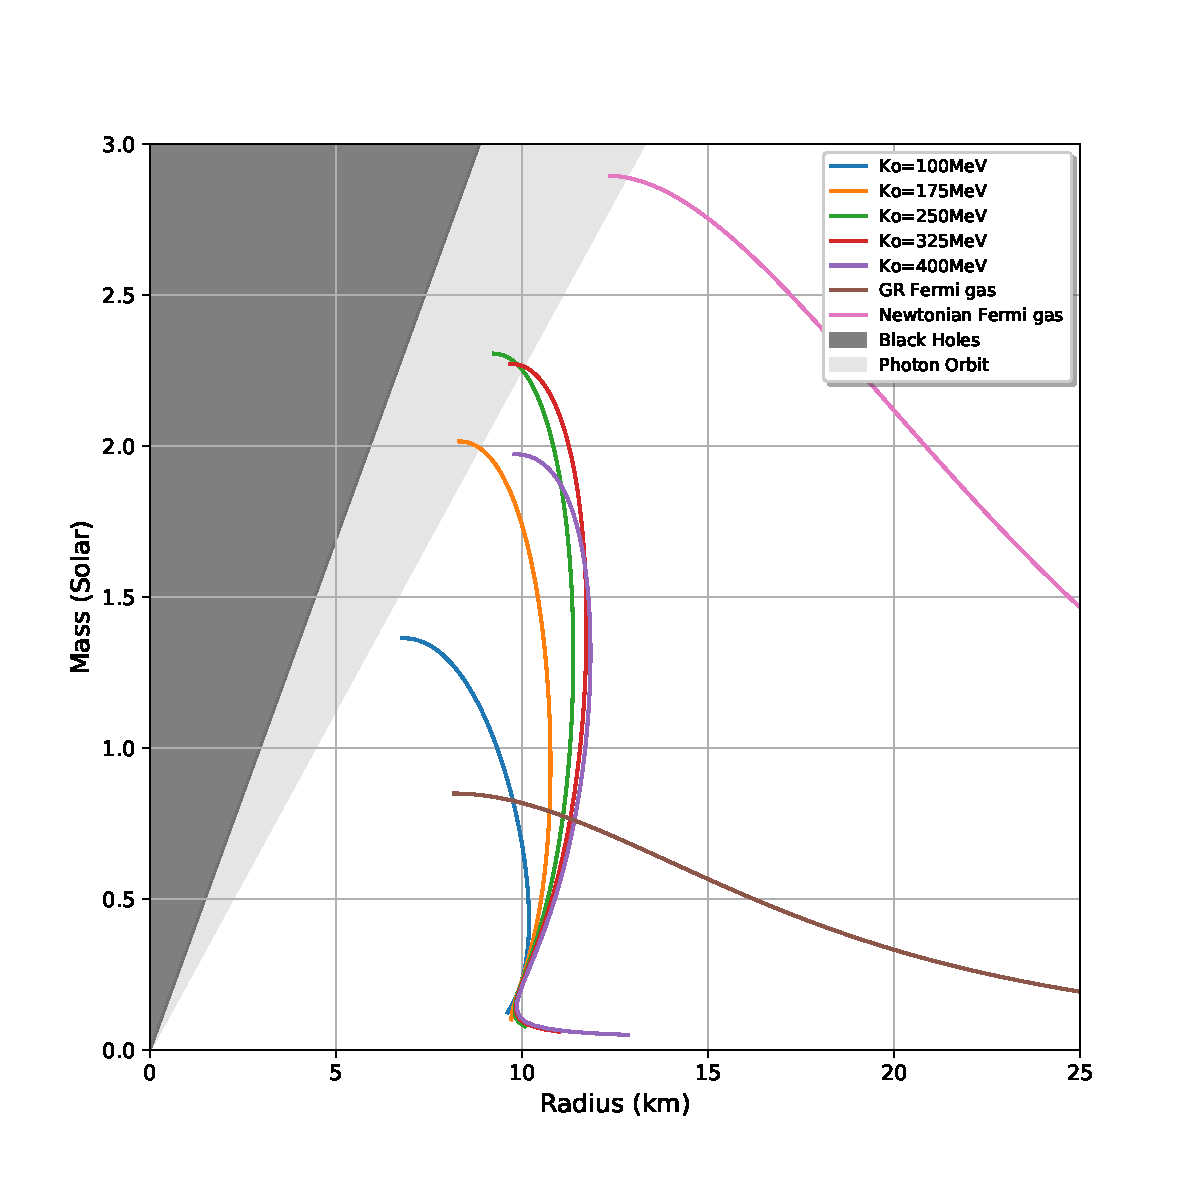
\includegraphics[scale=0.3]{eos_compare_our_model.pdf}
    \caption{Comparison between Fermi gas with Newtonian structure, General Relativistic structure, and model with nucleon interactions of different stiffness ($K_{0}$).}\label{fig/ourmodel}
  \end{figure}
\end{frame}

\begin{frame}
 \frametitle{Comparison with models from the literature}
 \begin{figure}
    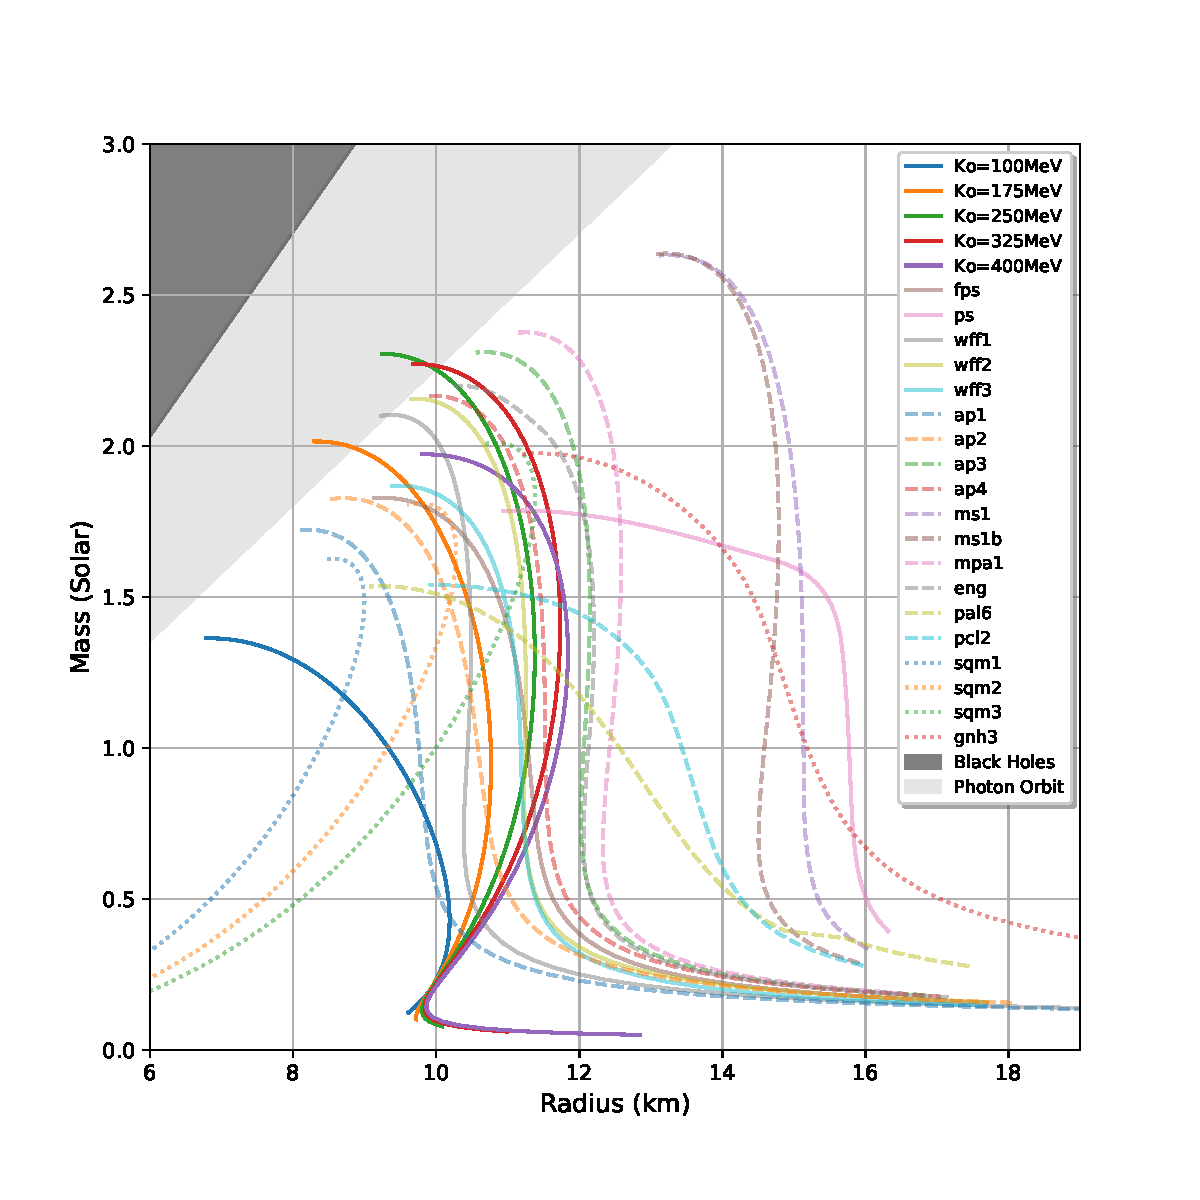
\includegraphics[scale=0.3]{eos_compare_paper.pdf}
    \caption{Comparison between Fermi gas model with nucleon interactions to other EOS models in the literature.}
 \end{figure}
\end{frame}

\begin{frame}
 \frametitle{Comparison with observation data}
 \begin{figure}
    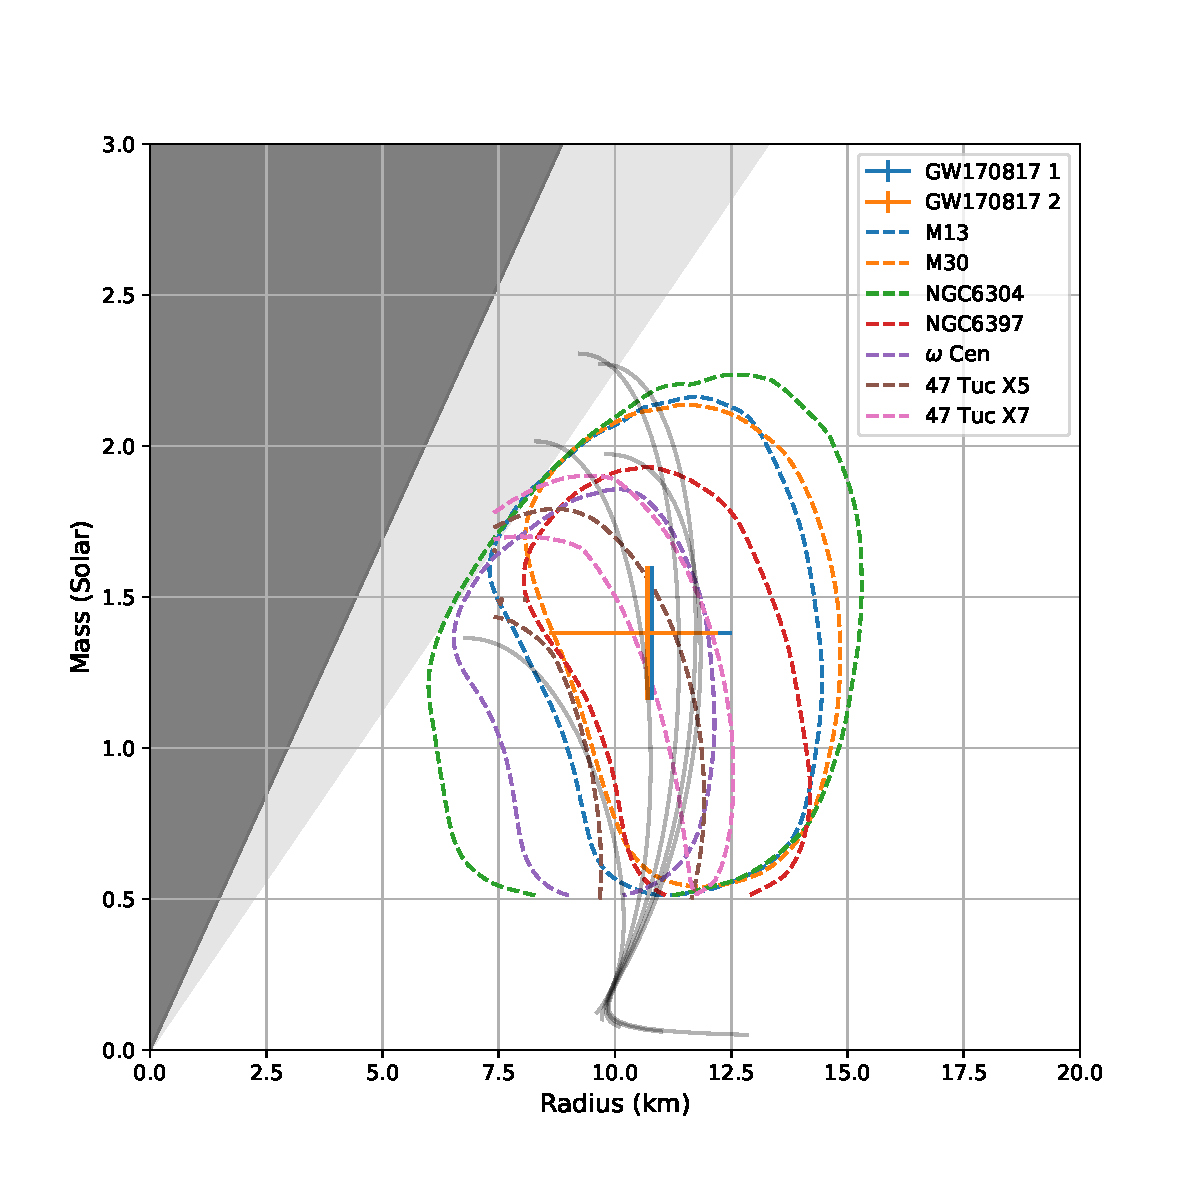
\includegraphics[scale=0.3]{eos_compare_obsv1_GW.pdf}
    \caption{Comparison between our models with observations from quiescent low mass X-ray binaries and gravitational wave event.}
 \end{figure}
\end{frame}

\begin{frame}
 \frametitle{Comparison with observation data}
 \begin{figure}
    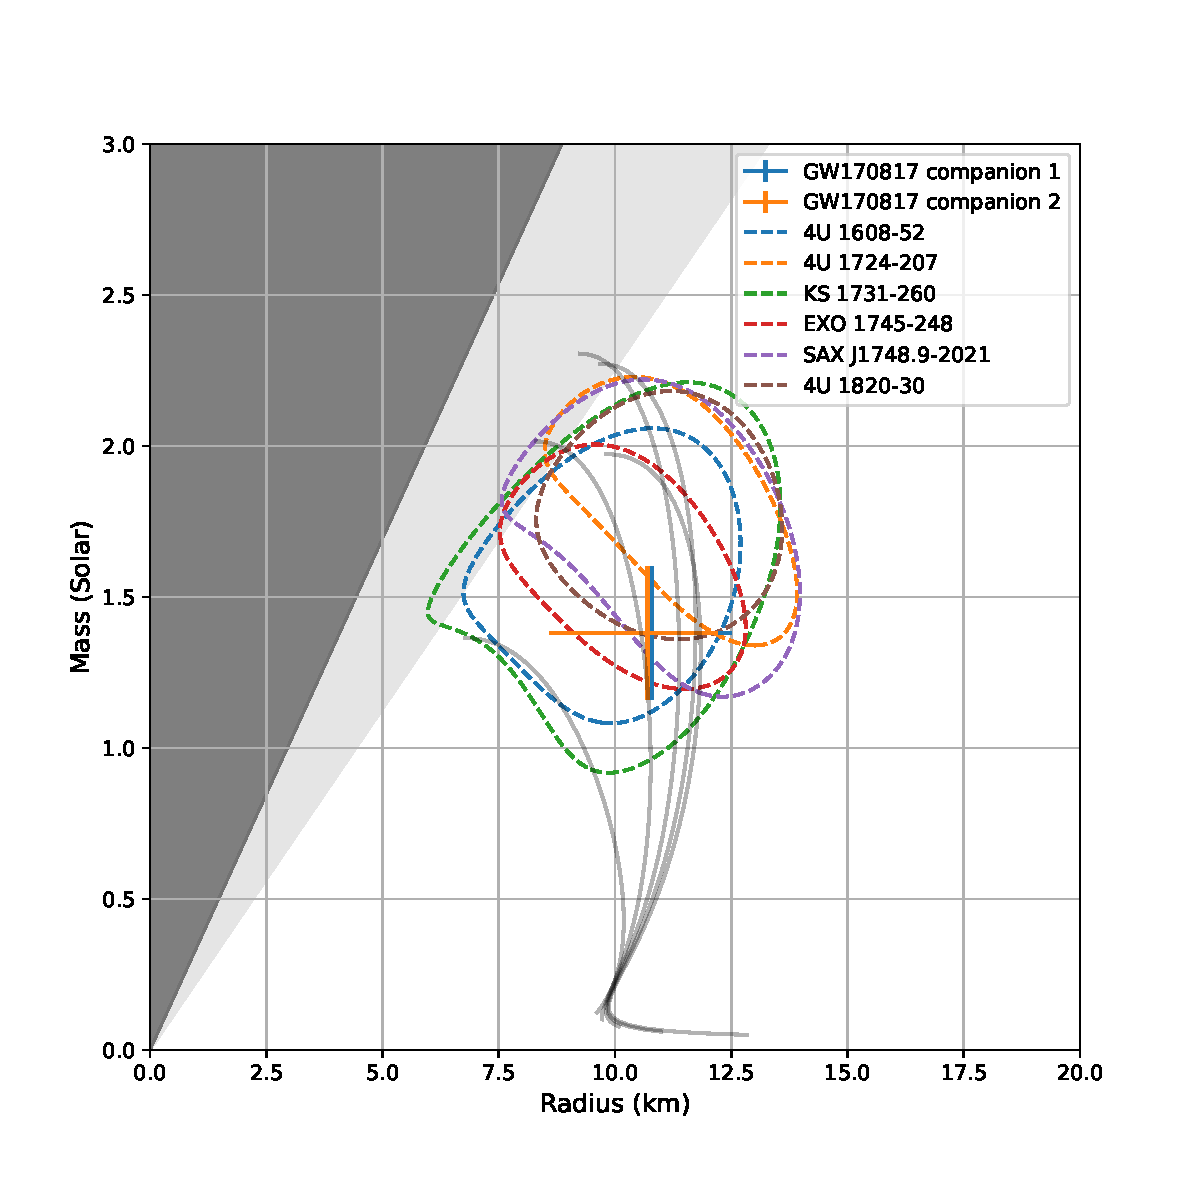
\includegraphics[scale=0.3]{eos_compare_obsv2_GW.pdf}
    \caption{Comparison between our models with observations from thermonuclear bursts of LMXBs and gravitational wave event.}
 \end{figure}
\end{frame}

\end{document}
